\section{Анализ предметной области}
\subsection{Принцип работы программно-информационной системы управления обучением}

В условиях глобализации образовательных процессов и роста числа иностранных студентов, изучающих программирование, возникает потребность в специализированных программных системах, обеспечивающих поддержку самостоятельного обучения. Согласно международным стандартам качества образования, такие системы должны предоставлять доступ к учебным материалам, автоматизировать проверку знаний и учитывать языковые особенности пользователей. Веб-приложение для компьютерной поддержки самостоятельной работы иностранных студентов при изучении языка программирования JavaScript позволяет автоматизировать ключевые процессы обучения. Рассмотрим основные из них:

\subsubsection{Управление курсами}
После создания курса преподавателем через интерфейс системы, он становится доступным для записи студентов. Курс включает уроки и тесты, которые автоматически отображаются в панели студента. Студент может записаться на курс, просмотреть его содержание и начать обучение. Система фиксирует прогресс студента, а данные о записи передаются в базу данных SQLite для дальнейшей аналитики.

\subsubsection{Управление уроками}
Преподаватели могут добавлять уроки через форму, редактировать их и сортировать с помощью Sortable.js. Каждый урок содержит описание, материалы и тесты. Система автоматически проверяет доступность урока для студента: доступ к следующему уроку открывается только после выполнения теста предыдущего урока. Уроки поддерживают локализацию через Django i18n, что позволяет иностранным студентам выбирать язык интерфейса.


\subsubsection{Управление тестами}
Система автоматизирует создание и управление тестами. Преподаватель может добавлять вопросы и ответы, указывать правильные варианты и проходной балл. Студенты проходят тесты через интерфейс урока, а система автоматически подсчитывает баллы и фиксирует результаты. Для иностранных студентов предусмотрена локализация вопросов и ответов, что упрощает процесс тестирования.

\subsubsection{Аналитика и результаты}
Для анализа успеваемости студентов система предоставляет модуль управления результатами. Преподаватель может просматривать результаты тестов, включая средний балл, максимальный и минимальный, а также удалять их при необходимости. Студенты получают доступ к своим результатам через панель, что позволяет отслеживать прогресс. Данные хранятся в базе SQLite и доступны для аналитики. 

\subsubsection{Поддержка пользователей} 
Система включает модуль управления пользователями, который поддерживает регистрацию студентов и преподавателей. Для иностранных студентов предусмотрена смена языка интерфейса через Django i18n, что обеспечивает комфортное использование. Также система фиксирует роли пользователей и ограничивает доступ к функционалу через декораторы.


\subsection{Компоненты программно-информационной системы управления обучением}
Программно-информационная система управления обучением представляет собой комплекс взаимодействующих программных модулей, аппаратных средств и технологий, предназначенных для хранения, обработки и предоставления образовательного контента. Важным условием функционирования системы является наличие интернет-соединения, обеспечивающего взаимодействие между клиентской и серверной частями. Для обеспечения безопасности данных используется аутентификация через Django contrib.auth, а также защита маршрутов (@loginrequired). На рисунке ~\ref{system:image} представлена схема взаимодействия компонентов системы управления обучением, а также способы их взаимодействия. 

\begin{figure}[ht]
	\centering
	\center{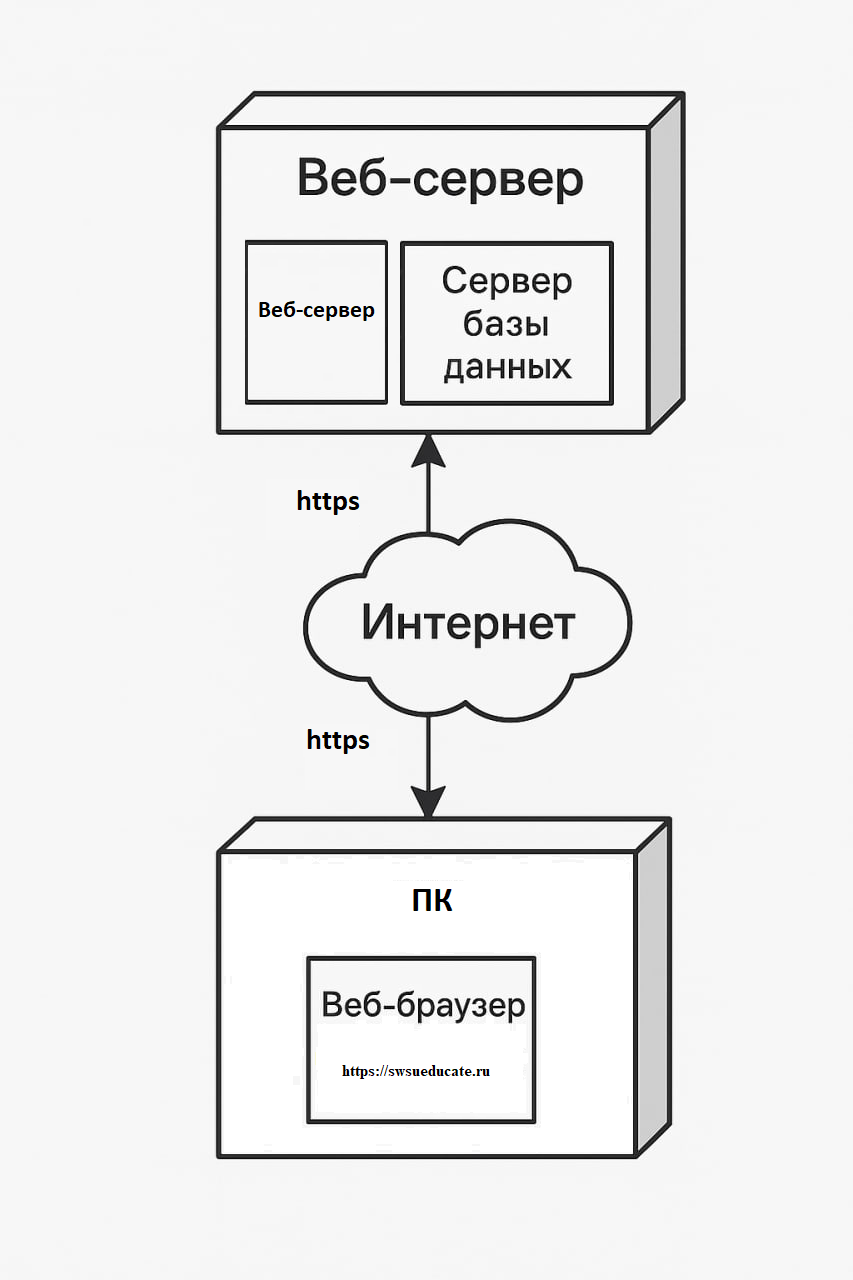
\includegraphics[width=0.6\linewidth]{images/диаграмма2}} 
	\caption{Схема взаимодействия компонентов системы управления обучением}
	\label{system:image}
\end{figure}


\subsection{Отчёты успеваемости}
Одной из причин использования веб-приложения в образовательных целях является удобство формирования отчётов об успеваемости. В системе предусмотрен модуль аналитики, в котором представлена статистическая информация для таких категорий, как прогресс студентов, результаты тестов и активность пользователей. Рассмотрим ключевой отчёт:

\subsubsection{Отчёт по результатам тестов}
Отчёт по результатам тестов представляет собой документ, фиксирующий итоги выполнения тестов студентами за определённый период. Он формирует данные о баллах на момент начала и завершения теста, сведения об общем количестве попыток (attemptnumber), информацию о проходном балле, а также статистику: средний, максимальный и минимальный балл. Пример отчёта представлен на рисунке. 

\begin{figure}[ht]
	\centering
	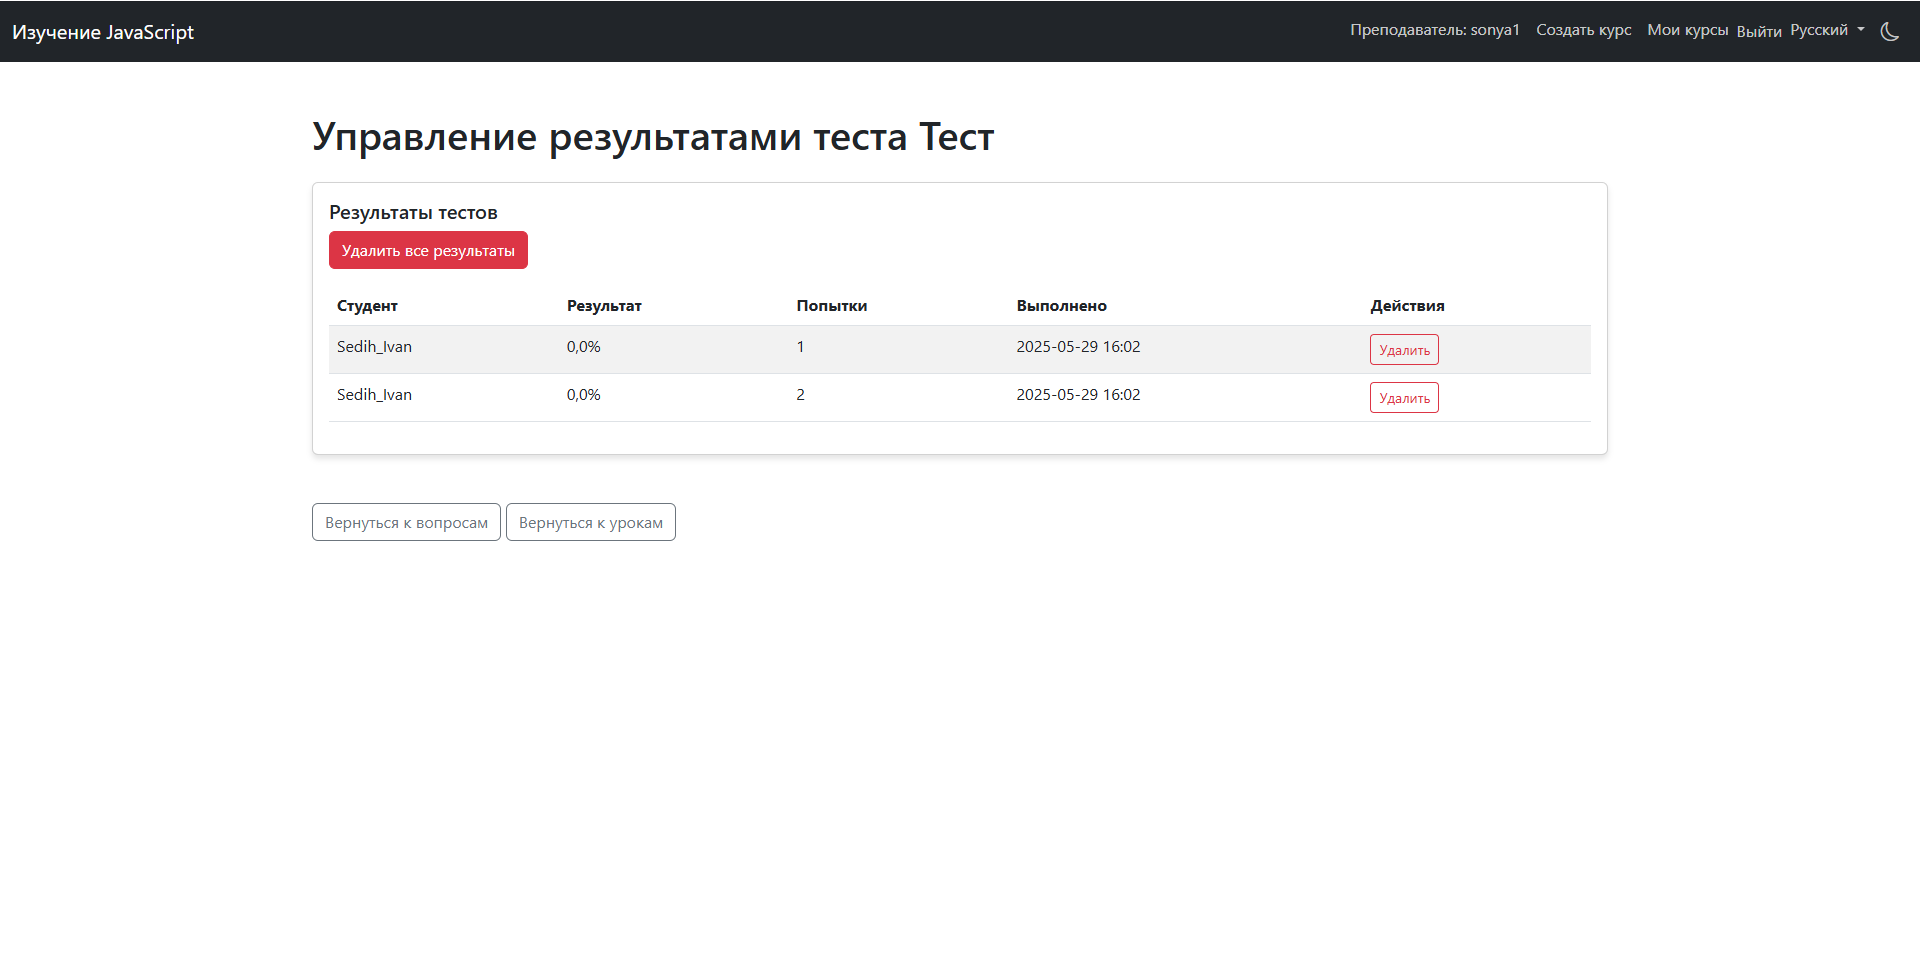
\includegraphics[width=1\linewidth]{images/резы} 
	\caption{Отчёт по результатам тестов}
	\label{zotchet:image}
\end{figure}

Ключевой особенностью данного отчёта является ограничение на количество попыток прохождения теста. Если студент превышает допустимое число попыток, доступ к тесту блокируется, и система уведомляет об этом (messages.error). Каждому отчёту присваивается уникальный идентификатор, исключающий дублирование данных при формировании статистики за определённый период.

Поскольку результаты тестов фиксируются в базе данных SQLite, отчёт не подлежит обнулению или повторному формированию без вмешательства администратора. Данные о результатах автоматически передаются преподавателю через интерфейс (managetestresults), что упрощает анализ. 

Отчёт по результатам тестов необходим: 

\begin{itemize}
	\item студенту для отслеживания своего прогресса и улучшения результатов; 
	\item преподавателю для контроля успеваемости и корректировки учебного плана; 
	\item администратору системы для анализа активности пользователей и проверки корректности работы модуля тестирования.
\end{itemize}

\subsection{Сравнительный анализ аналогичных систем}

Для оценки разработанной системы рассмотрим аналогичные платформы управления обучением, сравним их функциональность и определим конкурентные преимущества.

\subsubsection{Примеры аналогичных систем}

\begin{enumerate}
	\item {Moodle.} Moodle --- популярная открытая LMS, используемая в образовательных учреждениях. Она поддерживает создание курсов, тестирование и управление пользователями через модульную архитектуру.
	\item {Canvas LMS.} Canvas --- коммерческая LMS, ориентированная на образовательные учреждения и корпоративное обучение. Известна интуитивным интерфейсом и интеграцией с внешними инструментами (Google Drive, Zoom).
	\item {Google Classroom.} Google Classroom --- бесплатная платформа от Google для упрощённого обучения. Интегрируется с экосистемой Google, но подходит скорее для школ и небольших групп.
\end{enumerate}

\subsubsection{Сравнение функциональности}

\begin{xltabular}{\textwidth}{|p{3.1cm}|p{3.1cm}|p{3.5cm}|X|}
	\caption{Сравнение функциональности систем управления обучением\label{comparison:table}}\\ \hline
	Функция & Система & Описание & Дополнительные замечания \\ \hline
	\endfirsthead
	\continuecaption{Продолжение таблицы \ref{comparison:table}}\\ \hline
	Функция & Система & Описание & Дополнительные замечания \\ \hline
	\endhead
	Управление курсами & Разработанная система & Создание курсов, запись студентов, отслеживание прогресса (courses\_enrol-lment). & Простая структура хранения. \\ \hline
	Управление курсами & Moodle & Курсы с категориями и ролями. & Сложная иерархия. \\ \hline
	Управление курсами & Canvas LMS & Гибкие настройки доступа, модули. & Интеграция с внешними инструментами. \\ \hline
	Управление курсами & Google Classroom & Быстрое создание курсов, минимум опций. & Только базовые функции. \\ \hline
	
	Управление уроками & Разработанная система & Добавление уроков, сортировка по полю (order), прогресс через (courses\_prog-ress). & Контроль доступности. \\ \hline
	Управление уроками & Moodle & Уроки с медиа и интерактивом. & Широкий функционал. \\ \hline
	Управление уроками & Canvas LMS & Модульная структура, поддержка мультимедиа. & Гибкая система. \\ \hline
	Управление уроками & Google Classroom & Уроки как задания. & Ограниченная настройка. \\ \hline
	
	Управление тестами & Разработанная система & Создание тестов, локализация, подсчёт баллов (courses\_test, courses\_question). & Поддержка разных языков. \\ \hline
	Управление тестами & Moodle & Типы вопросов, разветвлённая аналитика. & Гибкая система оценивания. \\ \hline
	Управление тестами & Canvas LMS & Автоматизация и интеграции. & Расширенные возможности. \\ \hline
	Управление тестами & Google Classroom & Тесты через Google Forms. & Простой интерфейс. \\ \hline
	
	Аналитика и результаты & Разработанная система & Отчёты: средний, макс./мин. баллы (courses\_test-result). & Основной набор аналитики. \\ \hline
	Аналитика и результаты & Moodle & Расширенные отчёты, экспорт, группировка. & Удобно для ВУЗов. \\ \hline
	Аналитика и результаты & Canvas LMS & Визуализация результатов. & Графики, интерактивность. \\ \hline
	Аналитика и результаты & Google Classroom & Базовая статистика. & Ограниченный функционал. \\ \hline
	
	Локализация & Разработанная система & Интерфейс и контент через Django i18n. & Многоязычная поддержка. \\ \hline
	Локализация & Moodle & Поддержка языков через плагины. & Требует настройки. \\ \hline
	Локализация & Canvas LMS & Интерфейс локализован, контент частично. & Неполная поддержка. \\ \hline
	Локализация & Google Classroom & Интерфейс от Google, контент не локализуется. & Только интерфейс. \\ \hline
	
	Поддержка пользователей & Разработанная система & Регистрация, роли (isteacher, isstudent), доступ через (login\_required). & Простая авторизация. \\ \hline
	Поддержка пользователей & Moodle & Пользователи, группы, LDAP. & Подходит для больших структур. \\ \hline
	Поддержка пользователей & Canvas LMS & SSO, управление пользователями. & Высокая безопасность. \\ \hline
	Поддержка пользователей & Google Classroom & Аккаунты Google, базовые роли. & Простое управление. \\ \hline
\end{xltabular}




\subsubsection{Сравнительный анализ}

{Управление курсами и уроками.} Разработанная система обеспечивает базовые функции управления курсами и уроками с автоматическим контролем доступа, что подходит для самостоятельного обучения. Moodle и Canvas предлагают более сложные инструменты (категории, модули), но их сложность может быть избыточной для разработанной платформы. Google Classroom проще, но не поддерживает зависимости между уроками.

{Управление тестами.} Разработанная система выделяется локализацией вопросов и ответов, что важно для иностранной аудитории. Moodle и Canvas поддерживают больше типов вопросов (например, эссе), но требуют больше времени на настройку. Google Classroom ограничен Google Forms, что менее гибко.

{Аналитика.} Разработанная система предоставляет базовые отчёты, достаточные для небольшой платформы. Moodle и Canvas предлагают более мощную аналитику (графики, экспорт), но это может быть избыточным. Google Classroom уступает по аналитическим возможностям.

{Локализация.} Локализация через Django i18n делает разработанную систему удобной для пользователей с разными языками, особенно в части вопросов тестов. Moodle требует дополнительных пакетов для переводов, а Canvas и Google Classroom ограничены локализацией интерфейса.

{Поддержка пользователей.} Разработанная система использует Django contrib.auth для базовой аутентификации. Moodle и Canvas предлагают сложные механизмы (SSO, LDAP), которые могут быть избыточными. Google Classroom ограничивается Google Accounts.

\subsubsection{Преимущества и недостатки разработанной системы}

{Преимущества:}
\begin{itemize}
	\item локализация вопросов и ответов тестов через Django i18n;
	\item простота управления уроками с автоматическим доступом по прогрессу;
	\item лёгкая интеграция с SQLite для хранения и аналитики данных;
	\item простая и интуитивная система управления пользователями.
\end{itemize}

{Недостатки:}
\begin{itemize}
	\item ограниченные аналитические возможности (нет графиков, экспорта данных);
	\item отсутствие поддержки сложных типов вопросов (например, эссе);
	\item нет интеграции с внешними инструментами (например, Zoom, Google Drive).
\end{itemize}

\subsubsection{Выводы}

Разработанная система эффективно решает задачи управления обучением, предлагая удобный интерфейс, локализацию и автоматизацию. Для конкуренции с Moodle или Canvas можно добавить расширенную аналитику и поддержку сложных типов вопросов. Google Classroom уступает в гибкости, что делает разработанную платформу более подходящей для узкоспециализированных образовательных задач.



